\documentclass[11pt]{article}

\usepackage{themeKonstanz}

% Thesis information  %
\date{\today}
\year{2022}
\author{Fabian Klopfer}
\title{[WIP] Multi-Electrode Array \\ Standard Operating Procedure}

\headFoot{14}

\bibliography{resources}


\begin{document}
\thesistitlepage[language=english]


\begin{abstract}
 This standard operating procedure is supposed to provide information on the basic requirements and steps to be undertaken in order to record data from acute slices using the multi electrode array setup. \\

Much of the below is refering the reader to or adapted from the MultiChanel Systems MEA Application Note on
Acute Hippocampus Slices from Rat or Mouse~\cite{mcs}, the Axion Biosystems Acute Brain Slice Protocol~\cite{axion}, peer-reviewed protocols~\cite{star},\cite[chapter~6]{dallas2021patch} and the LAS interactive course on animal handling\cite{las}.
All manuals are linked in the citation, i.e. if you click the link, you'll download the document.
The peer-reviewed protocols are very detailed, the notes by MCS however are also very detailed.
Another source for this is the instructions that I received by Nikolas Layer and Daniela Miely.
\end{abstract}


\tableofcontents
\newpage

\section{Setup}
    General documentation on this can be found in the MEA2100-System: Installation Guide brochure by MCS~\cite{2100-install}, CMOS-MEA5000-System: Quickstart~\cite{5000-quick}, or in the respective user manuals~\cite{2100-man, 5000-man}. \\

    The Setup for the CMOS and the 256 MEA are very similar. The only difference is that the chip and the head stage have to be swapped (2100-256 and 5000-CMOS), as well as the recording software used. \\

    Detailed handling instructions for the chips, like coating, cleaning and storage can be found in the MCS MEA manual~\cite{mea-man}. \\

    \textbf{Components:}
    \begin{itemize}
     \item MEA-Chip (256MEA or CMOS-MEA; SCB or SCA for slices, CC for cell culture. For more details see the respective chip datasheets)
     \item MEA-Headstage (2100 for 256 or 5000 for CMOS)
     \item Interface board MCS-IFB-C 3.0 Multiboot
     \item MEA-to-interface board Connector cable (iX-industrial cable, type B)
     \item Temperature controller (TC02)
     \item Perfusion Cannula (PH01)
     \item Peristaltic perfusion system (PPS2)
     \item Video-Microscope
     \item Light source for the microscope
     \item Controls for the microscope
    \end{itemize}

    For chemical stimulation, an additional stand and a puffing electrode is neccessary~\cite{puff-csd}.
    For meassuring concentrations and DC two micromanipulators and electrodes are neccessary, one of which must be prepared specifically.

    TODO add pictures

\section{Preparation}
    \subsection{Artificial Cerebrospinal Fluid}
        Recipies for aCSF can also be found in \cite[p. 10]{star}, \cite[p. 122]{dallas2021patch} and \cite{mcs}.
        Example for recording FHM3 CSDs: \\
        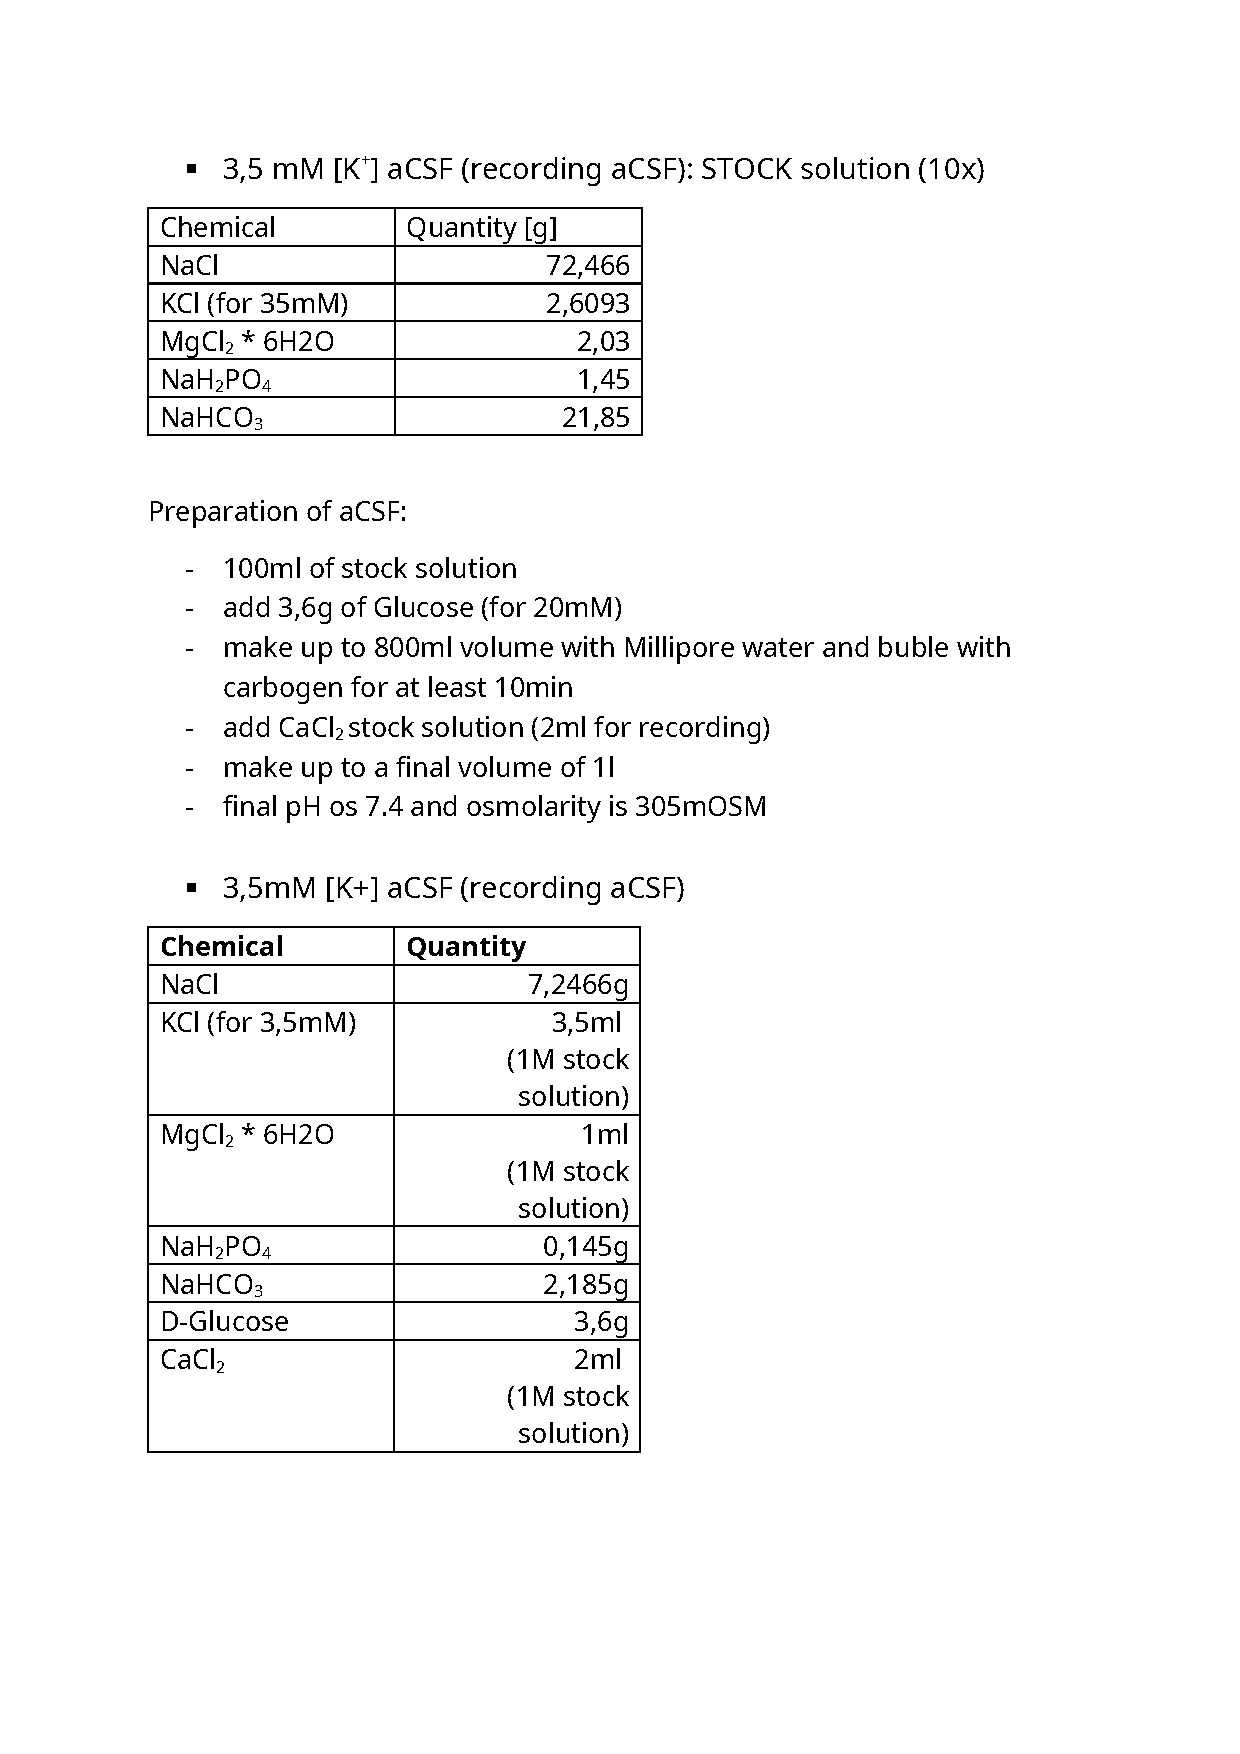
\includegraphics[keepaspectratio,width=\textwidth]{img/aCSF_3.5mM_Potassium.pdf}

    \subsection{Acute Slices}
        For getting tissue, you should talk to your PI, if you don't have that already. \\
        If you have an animal, the steps to produce slices are described in detail in \cite[p. 10]{star}, \cite[p. 122]{dallas2021patch} and \cite{mcs}.

\section{Recording Steps}
    More detailed instructions and protocols can be found in \cite[p. 10]{star}, \cite[p. 122]{dallas2021patch}, \cite{axion} and \cite{mcs}.
    \begin{enumerate}
     \item Turn on Devices: Pump, interface board, light source, video microscope, computer, controler for microscope/micromanipulators
     \item Open Software: Pump, Temperature, Video Microscope, Multi Channel Experimenter
     \item Set-up pump: connect the tubes as outlined in the Installation guide (printer version in one of the two metal cases below the table to the right of the setup). Test the perfusion system and make sure that the waste's input is lower than the perfusions output in the chamber!
     \item Transfer and place slice: \cite{mcs} mentions, that the slice should be placed on the electrodes without liquid for a better establishment of contact between the electrodes and the tissue. I.e. place it with the transfer pipette, soak up the extra liquid with paper tissue and quickly start the perfusion to avoid damage to the tissue.
     \item Meassure: In the MC Experimenter, draw the mea headstage into the main area. Drag the recording tool to the main area. Connect the digital data from the headstage to the recorder. Double click the recorder. In the bottom of the window there is a tab ``data acquisition'' click it to see the windows for the graphs to be recorded. Press start DAQ to get graphs. Press record to actually record data.
     \item Clean \& Power off: Clean the tubes with distilled water and hang them up such that they can dry out and dont mold. Transfer your data to an external hard drive. Turn off all devices that you turned on. Rinse the MEA with VE water and dry it, in case you havent coated anything. Please look up the cleaning procedure neccessary in the MEA manual~\cite{mea-man}.
    \end{enumerate}

\section{Stimulation}
TODO
    \begin{enumerate}
     \item Chemical
     \item Electrical
    \end{enumerate}

\section{Analysis}
TODO



\newpage
\printbibliography
\end{document}
